\documentclass[11pt]{article}
\usepackage{graphicx}
\usepackage{float}
\usepackage{hyperref}
\usepackage{natbib}
\usepackage{listings}
\usepackage{xcolor}
\usepackage[dvipsnames]{xcolor}
\usepackage[svgnames]{xcolor}
\usepackage{amsmath} % For the equation* environment
\usepackage{amssymb}

\hypersetup{
    colorlinks=true,
    linkcolor=red,
    filecolor=cyan,      
    urlcolor=orange,
    pdftitle={Overleaf Example},
    pdfpagemode=FullScreen,
    }

\setlength{\textwidth}{6.5in}
\setlength{\headheight}{0in}
\setlength{\textheight}{8.0in}
\setlength{\hoffset}{0in}
\setlength{\voffset}{0in}
\setlength{\oddsidemargin}{0in}
\setlength{\evensidemargin}{0in}

\lstdefinestyle{txtstyle}{
    basicstyle=\ttfamily\small,
    breaklines=true,
    backgroundcolor=\color{Bisque}
}
\lstset{style = txtstyle}

\definecolor{codegreen}{rgb}{0,0.6,0}
\definecolor{codegray}{rgb}{0.5,0.5,0.5}
\definecolor{codepurple}{rgb}{0.58,0,0.82}
\definecolor{backcolour}{rgb}{0.95,0.95,0.92}

\lstdefinestyle{mystyle}{
    backgroundcolor=\color{backcolour},   
    commentstyle=\color{codegreen},
    keywordstyle=\color{magenta},
    numberstyle=\tiny\color{codegray},
    stringstyle=\color{codepurple},
    basicstyle=\ttfamily\footnotesize,
    breakatwhitespace=false,         
    breaklines=true,                 
    captionpos=b,                    
    keepspaces=true,                                   
    numbersep=5pt,                  
    showspaces=false,                
    showstringspaces=false,
    showtabs=false,                  
    tabsize=2
}

\title{Computational Physics ps-3 Report}
  
\author{Tongzhou Wang, \\ GitHub account: TZW56203, repository: phys-ga2000, \\ \url{https://github.com/TZW56203/phys-ga2000}}

\date{September 24, 2024}

\begin{document}

\maketitle

\section{Problem 1}
The relation between the matrix multiplication computation time and the matrix size ($N \times N$) is shown below.
\begin{figure}[H]
    \centering
    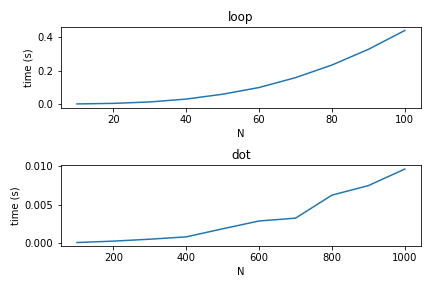
\includegraphics[scale = 1.0]{images/t-N.png}
    \caption{Matrix multiplication computation time vs matrix size.}
    \label{fig:t-N}
\end{figure}
\begin{figure}[H]
    \centering
    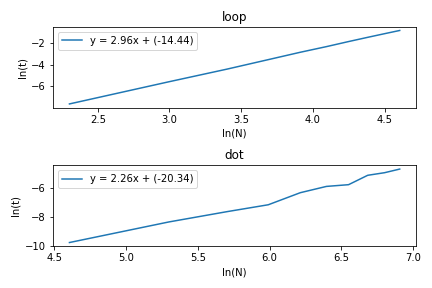
\includegraphics[scale = 1.0]{images/lnt-lnN.png}
    \caption{Logarithmic time vs logarithmic size.}
    \label{fig:lnt-lnN}
\end{figure}

The computation time of the loop function rises as $N^3$ as predicted. This can be concluded from Figure \ref{fig:lnt-lnN}, where we have for the loop function $\ln{(t)} = 2.96 \ln{(N)} - 14.44$. The coefficient 2.96 indicates that the computation time rises as $N^3$.

Similarly, we can conclude that the computation time of the dot function does not rises as $N^3$.

The main difference between the two function is that the dot function is much faster, which can be seen from Figure \ref{fig:t-N}.

\section{Problem 2}
\begin{figure}[H]
    \centering
    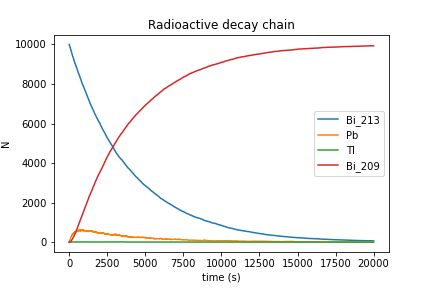
\includegraphics[scale = 1.0]{images/ps-3-2.png}
    \caption{Radioactive decay chain.}
\end{figure}

\section{Problem 3}
\begin{figure}[H]
    \centering
    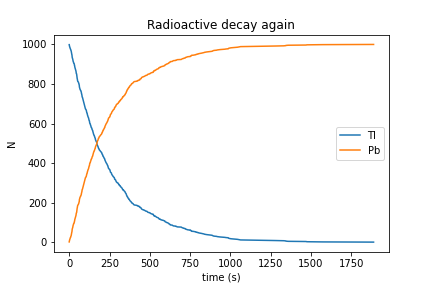
\includegraphics[scale = 1.0]{images/ps-3-3.png}
    \caption{Radioactive decay again.}
\end{figure}

\section{Problem 4}
To find the mean and variance of the random variable $y = N^{-1}\sum_{i=1}^{N} x_i$, we first look at the independent and identically distributed random variables $x_i$, which have probability density $f = e^{-x}$. It is straight forward to find the mean and variance of $x_i$.
\begin{equation}
\begin{gathered}
    \mu \equiv \mathbb{E}(x) = \int_0^\infty x e^{-x} dx = 1, \\
    \sigma^2 \equiv \mathrm{Var}(x) = \mathbb{E}(x^2) - \mathbb{E}^2(x) = 1.
\end{gathered}
\end{equation}

We then proceed to obtain
\begin{equation}
\begin{split}
    \mathbb{E}(y) = & \mathbb{E}\left( \frac{1}{N}\sum_{i=1}^{N} x_i \right) \\
    = & \frac{1}{N} \mathbb{E}\left( \sum_{i=1}^{N} x_i \right) \\
    = & \frac{1}{N} \sum_{i=1}^{N} \mathbb{E}(x_i) \\
    = & \frac{N \mu}{N} \\
    = & \mu = 1,
\end{split}
\end{equation}
and
\begin{equation}
\begin{split}
    \mathrm{Var}(y) = & \mathrm{Var}\left( \frac{1}{N}\sum_{i=1}^{N} x_i \right) \\
    = & \frac{1}{N^2} \mathrm{Var}\left( \sum_{i=1}^{N} x_i \right) \\
    = & \frac{1}{N^2} \sum_{i=1}^{N} \mathrm{Var}(x_i) \\
    = & \frac{N \sigma^2}{N^2} \\
    = & \frac{\sigma^2}{N} = \frac{1}{N}.
\end{split}
\end{equation}

Figure \ref{yhist} and \ref{zhist} visually show that for large $N$ the distribution of $y$ tends toward Gaussian. Here we define
\begin{equation}
    z = \frac{\sqrt{N} (y-\mu)}{\sigma},
\end{equation}
which according to the central limit theorem should have a standard normal distribution.

\begin{figure}[H]
    \centering
    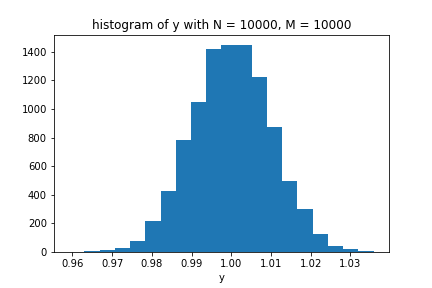
\includegraphics[scale = 0.8]{images/ps-3-4-yhist.png}
    \caption{Histogram of $y$.}
    \label{yhist}
\end{figure}

\begin{figure}[H]
    \centering
    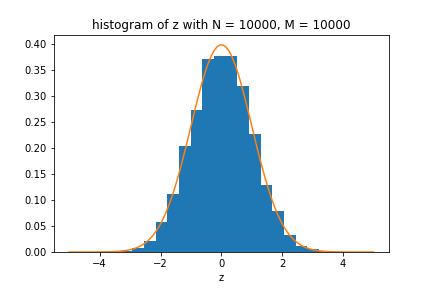
\includegraphics[scale = 0.8]{images/ps-3-4-zhist.png}
    \caption{Histogram of $z$.}
    \label{zhist}
\end{figure}

\begin{figure}[H]
    \centering
    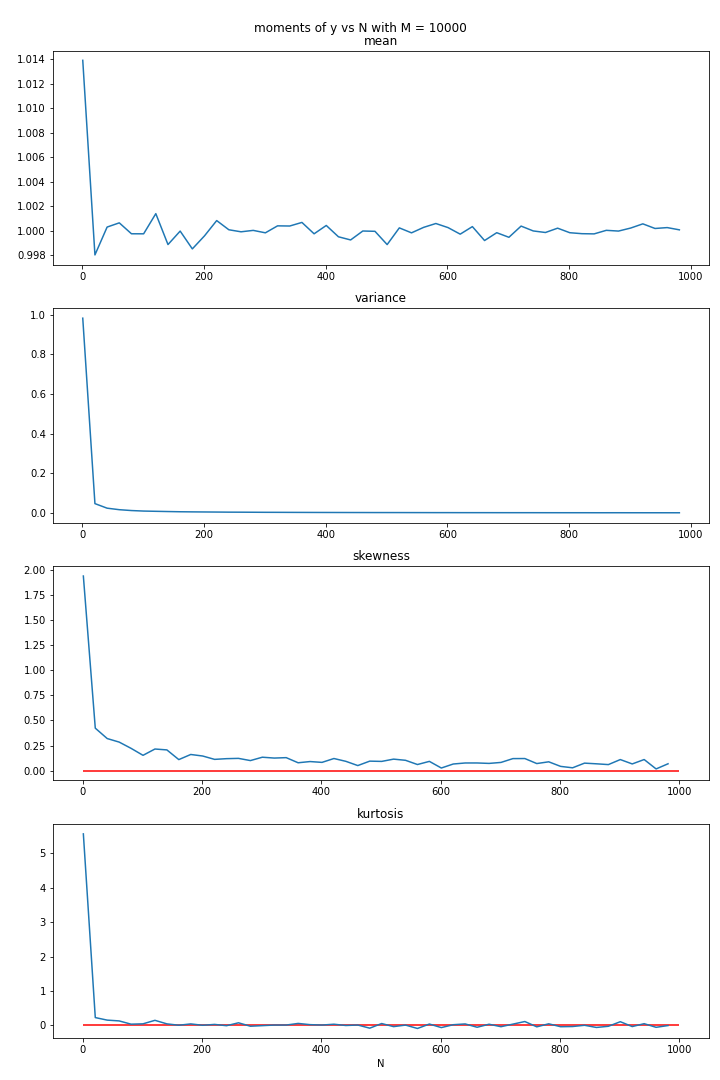
\includegraphics[scale = 0.55]{images/ps-3-4_moments.png}
    \caption{Moments of $y$ vs $N$.}
    \label{moments}
\end{figure}

Figure \ref{moments} shows the mean, variance, skewness, and kurtosis of $y$ as a function of $N$.

Around $N = 600$, the skewness reached about $1\%$ of its value at $N = 1$.

Around $N = 100$, the kurtosis reached about $1\%$ of its value at $N = 1$.

\end{document}
